\section{Evaluation}
\FloatBarrier%

To recap the previous sections, we are dealing with two models here:
\begin{itemize}
  \item ``WordCNN'', a convolutional neural network operating on tokenized words
    and punctuation,
  \item ``CharCNN'', a convolutional neural network operating on tokenized
    characters,
\end{itemize}
as well as three variations for each model:
\begin{itemize}
  \item No clustering.
  \item The data is augmented with K-Means clustering.
  \item The data is augmented with clustering through an infinite Gaussian
    mixture model.
\end{itemize}
These variations will be referred to as ``Baseline'', ``K-Means'' and ``GMM ''
respectively. Although K-fold cross validation is a common way of comparing
the performance of different, there are two reasons why it isn't used in these
experiments:
\begin{itemize}
  \item One of the more interesting variables in this context is the size of the
    training set, but with cross validation it is directly tied to the number of
    folds (e.g.\ with a dataset of 1000 samples and 10 folds, each fold
    would have a training set of 100 samples).
  \item The training set and the test set are sampled from the same pool of
    data. In our case, we want the training set and the test set to be sampled
    from different electoral periods, because:
    \begin{itemize}
      \item A change of electoral period means at least a partial change in
        parliamentary members, which reduces the ability of the model to 
        overfit on their names.
      \item Although older documents use the same layout as newer ones, the PDF
        files were generated using different software (electoral period 13 started
        in 1994 and was the first period to use truly  digital documents --- older
        documents are scanned versions of printed paper). Since PDF
        decompilation is already a flaky process, this results in the 
        PDF decompiler making different mistakes than it does on the newer
        documents. This is a big problem for rule-based systems, but hopefully the
        probabilistic nature of neural networks makes them more robust to this issue.
    \end{itemize}
\end{itemize}
Therefore, a variation of cross validation is used instead. There is a pool of
training data consisting of documents from the 18th electoral period of the
\emph{Bundestag}, and a test set containing documents from the
electoral periods \numrange{13}{17}.
For 10 iterations, $k$ samples are pulled from the pool of training data. Each
of the three models is trained on these samples and then tested on the full test
set.

\subsection{Results}
The results of the main experiments are shown in \cref{fig:results}.
A number of things are immediately noticeable:
\begin{itemize}
  \item With a context window of size 1 (i.e.\ only a single line of text),
    results are particularly bad. Adding the subsequent line of text (a window
    size of 2) increases performance significantly, but additional increases
    lead to diminishing returns and eventual regression in performance.
  \item The CharCNN model scales better with the size of the dataset than the
    TokenCNN model; in each case except for the smallest window size, TokenCNN
    has a much flatter curve. It outperforms CharCNN at low dataset sizes, but
    in most cases CharCNN manages to edge out a bit of extra performance at 2400
    and 3000 samples.
  \item GMM clustering performs equal to or better than the baseline in almost
    every case; in some cases the GMM curve is clearly above the baseline curve,
    in others they are close enough that their confidence interval overlaps.
    K-Means clustering is a little bit harder to pin down, but in many cases
    seems to fall in between the baseline and GMM clustering.
\end{itemize}

\begin{figure}[tb]
  \centering
  \makebox[\textwidth]{
	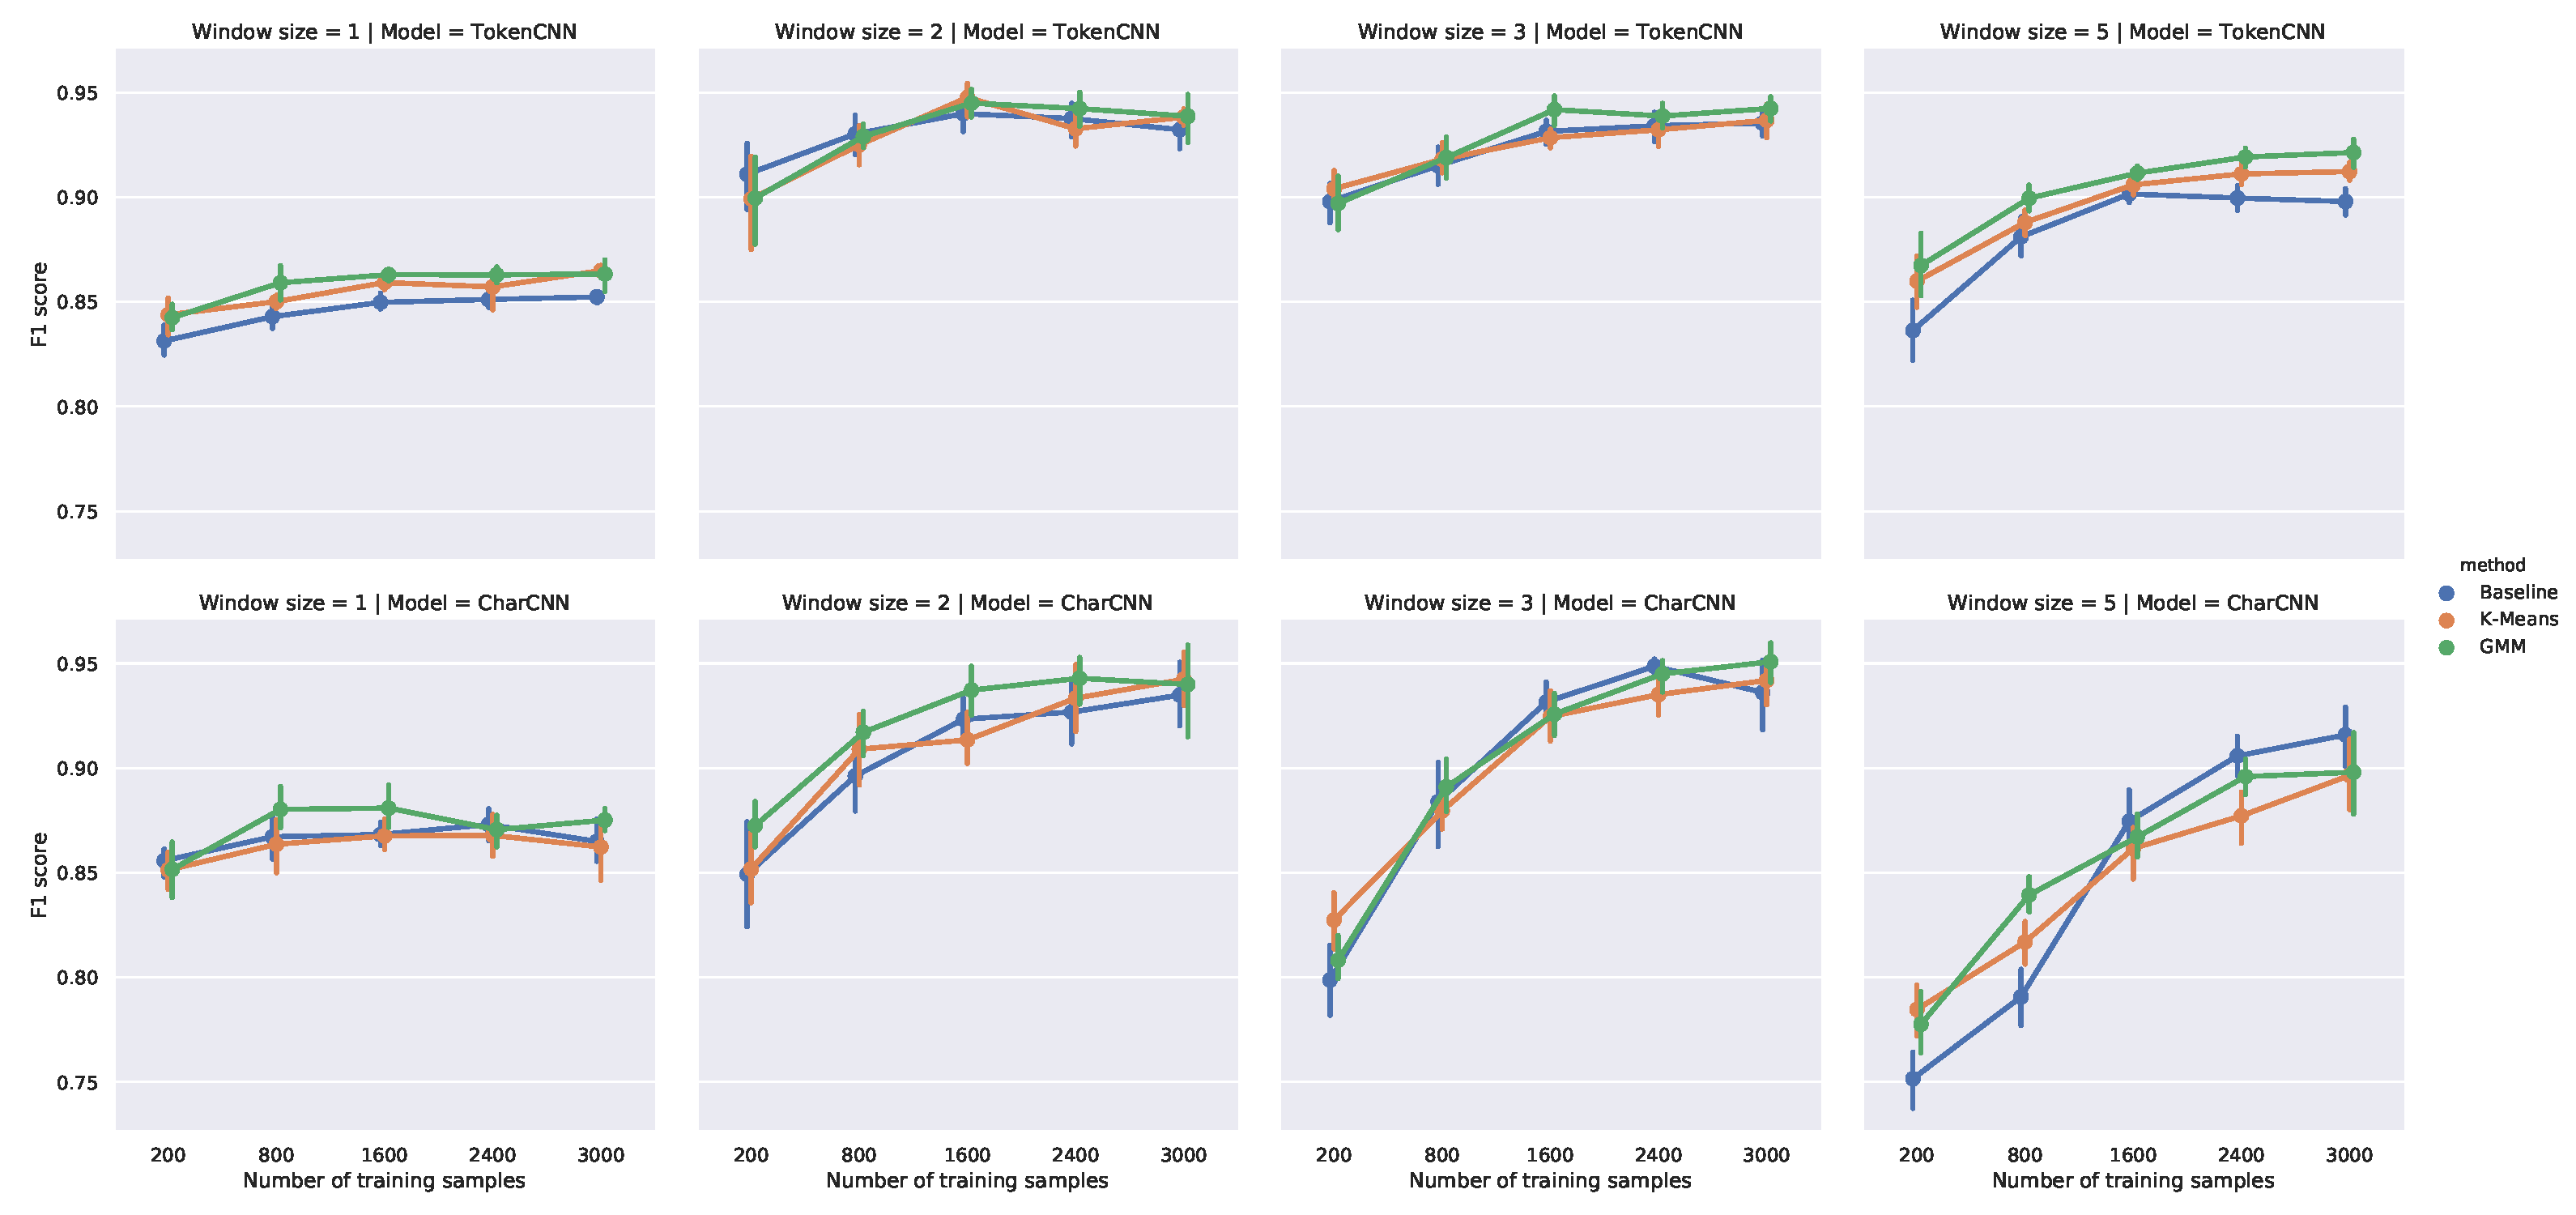
\includegraphics[width=\paperwidth]{figures/results/all_results.pdf}
  }
  \caption{A number of point plots showing the F1 scores of the experiments,
    averaged over 10 cross validation runs. The error bars indicate the 95\%
    confidence interval, meaning that the true mean has a 95\% chance of lying
    within the shown interval.  The number of training samples is varied on the
    x-axis; the left column shows the TokenCNN model, the right column the
    CharCNN model. The rows correspond to the size of the context window. The
    three clustering methods are displayed within the same
  graph.\label{fig:results}}
\end{figure}

It is risky to readily draw conclusions from this data, as the variance between
cross validation runs is high relative to the difference in F1 score between the
models. Although significance testing (by means of of P scores) can be a useful
tool in scenarios like this, their power with is relatively low with the low
sample size of 10 combined with the small difference in scores.  Increasing the
number of cross validation folds would have been a solution, although at
significant cost in both time and electricity; instead, the discriminative power
can be increased by coalescing the results at different parameter
configurations. This is shown in \cref{tbl:p_all} for all parameters, and in
\cref{tbl:p_best} for a well-performing subset of parameters. This paints a much
clearer picture. In \cref{tbl:p_all}, the TokenCNN model is significantly
improved by both forms of clustering, while the CharCNN does not appear to
benefit from adding K-Means clustering. In this overall case, the TokenCNN also
outperforms the CharCNN, mostly because of the inclusion of the low amounts of
training data which the CharCNN model struggles with.

Restricting our view to the better performing parameter settings in
\cref{tbl:p_best}, a couple of things change. First of all, K-Means clustering
does not appear to improve the scores for either model. GMM clustering is still
a significant improvement when applied to the TokenCNN. When applied to
the CharCNN, the score is still quite a bit higher, although it loses its
significance in a statistical sense. Additionally, CharCNN now wins out over
TokenCNN with a slight margin.

\subsection*{Discriminative power of clustering}
Now that it is somewhat established that GMM clustering outperforms K-Means
clustering, it might be interesting to look at their differences in greater
detail. We have already compared the baseline (only text) with the augmented
models (text and clustering); why not add something of an inverse baseline that
is trained using only the clustering data? The results of this experiment are
shown in \cref{fig:only_clusters}, and they contain some surprises. While the
previous experiments seemed to imply that adding GMM clustering improved the F1
scores more than adding K-Means clustering did, here we actually see K-Means on
its own significantly out-perform GMM at larger window sizes. In fact, K-Means
seems to scale very well with increased window sizes, while the GMM performance
is rather constant. In addition, K-Means suffers far less when lowering the
number of training samples to 200. Lastly, their performance is surprisingly
good. The peak F1 score of around 0.85 is not all that far removed from the
baseline scores of roughly 0.94, considering the amount of information discarded
in the text.

\begin{figure}[tb]
  \centering
  \makebox[\textwidth]{
	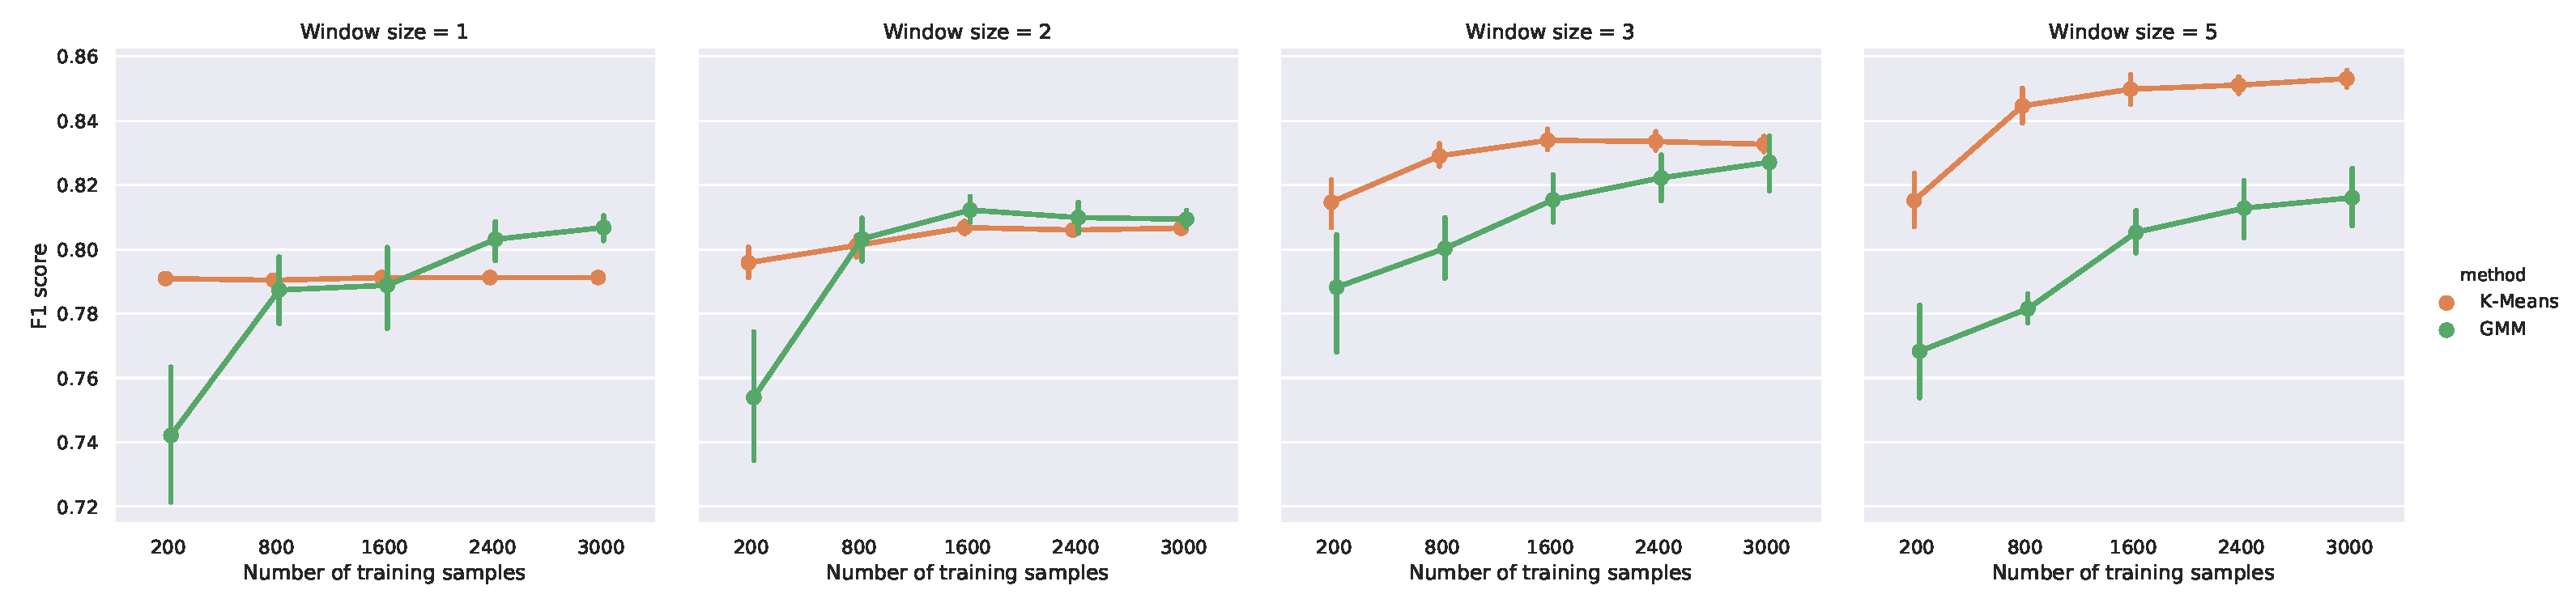
\includegraphics[width=\paperwidth]{figures/results/all_results_only_clusters.pdf}
  }
  \caption{This figure is similar to \cref{fig:results}, except when trained on
	\emph{only} the clustering data, with the textual data being
	discarded.\label{fig:only_clusters}}
\end{figure}


\begin{table}[tb]
  \begin{subfigure}[b]{\textwidth}
    \centering
    \begin{tabular}{lrrrr}
      \toprule
      & \multicolumn{2}{c}{TokenCNN} & \multicolumn{2}{c}{CharCNN}\\
      \cmidrule(lr){2-3} \cmidrule(lr){4-5}
      Method   & Mean  & P              & Mean  & P\\
      \midrule
      Baseline & 0.895 & -              & 0.880 & - \\
      K-Means  & 0.901 & \num{2.55e-05} & 0.880 & 0.81 \\
      GMM      & 0.905 & \num{6.12e-13} & 0.888 & \num{1.16e-04} \\
      \bottomrule
    \end{tabular}
    \caption{The values in this table are taken from all window sizes and all
    dataset sizes.\label{tbl:p_all}}
    \vspace*{1em}
  \end{subfigure}
  \begin{subfigure}[b]{\textwidth}
    \centering
    \begin{tabular}{lrrrr}
      \toprule
      & \multicolumn{2}{c}{TokenCNN} & \multicolumn{2}{c}{CharCNN}\\
      \cmidrule(lr){2-3} \cmidrule(lr){4-5}
      Method   & Mean  & P    & Mean  & P\\
      \midrule
      Baseline & 0.935 & -    & 0.937 & - \\
      K-Means  & 0.935 & 0.96 & 0.938 & 0.72 \\
      GMM      & 0.941 & 0.03 & 0.945 & 0.12 \\
      \bottomrule
    \end{tabular}
    \caption{The values in this table are taken from the best performing
    subset of the parameters, with the number of training samples being 2400 and
    3000 and the size of the context window set to 1 or 2.\label{tbl:p_best}}
  \end{subfigure}
  \caption{The results averaged over all tested parameters. The P column shows
    the P value comparing each model to the baseline, using a paired
    Student's t-test over the full cross validation output. The P value is based
    on the null hypothesis that neither model improves on the baseline. Using
    the common $P \leq 0.05$ cutoff for rejecting the null hypothesis, any P
    value below 0.05 would be grounds to consider the model to perform
    differently from the baseline. Since each model's mean score is equal to or
    higher than the baseline score, in this case we can fortunately take
    ``differently'' to mean ``better''.
  \label{tbl:results}}
\end{table}

\FloatBarrier%

%%% Local Variables:
%%% mode: latex
%%% TeX-master: "report"
%%% End:
